%% parked.tex -- corrected after the vLLM hardware validation
\documentclass[sigconf,nonacm]{acmart}
\microtypesetup{expansion=false}
\usepackage{xspace,booktabs,amsmath,amssymb,graphicx}
\newcommand{\sys}{\textsc{ParkAware}\xspace}
\newcommand{\code}[1]{\texttt{\small #1}}

\begin{document}

\title{Parked, but Reclaimable: Measuring the Missing State in\
Agentic LLM Autoscaling}
\author{Anonymous Author(s)}
\affiliation{\institution{Submission \#xxx}\country{}}

\begin{abstract}
Agent programs alternate model invocations with tool calls. During a tool
call, GPU utilisation and request queues can both be zero even though the
program will soon reuse a long prefix. We initially assumed that native vLLM
reserved that program's KV blocks and that KV-cache utilisation therefore
exposed the parked state. A hardware validation falsified this premise. In
vLLM~0.25.1, a completed request releases its blocks to a reclaimable prefix
cache: an immediate reuse may be cheap, but the exported active-KV metric also
reads zero and new work can evict the prefix.

We report the measurement, correct a trace-driven simulator, and re-evaluate
seven autoscaling policies. On Qwen2.5-14B, a 32k-token cache miss adds 9.03~s
relative to a hit, while all eight parked sessions produce zero GPU, running,
waiting, and active-KV readings in 114 samples. A pressure experiment shows
that a 16k prefix remains intact behind at most eight concurrent 4k contexts,
is about 64.5\% retained behind 16, and is gone behind 24; delays of 0--32~s
have little independent effect. The same run calibrates batching
($k_{1/2}=4.606$) and a 38.155~s process cold start.

The correction reverses the original policy result. Across six agentic points
on the Azure coding trace, mean SLO attainment is 0.935 for HPA, 0.931 for
KV-util, and 0.909 for a candidate policy that counts parked programs. Prefix
pressure, not scale-in alone, dominates recomputation, and the relative order
changes with cache capacity and batch size. The useful signal is therefore not
``parked occupancy'' but the uncertain future value and survival probability
of reclaimable prefixes. We release the falsified version, raw measurements,
corrected simulator, and negative result together.
\end{abstract}

\keywords{LLM serving, agents, autoscaling, prefix cache, negative results}
\maketitle

\section{Introduction}

An LLM agent is a program rather than a request. It invokes a model, runs an
external tool, appends the result, and invokes the model again on an extended
transcript~\cite{react}. Between invocations it uses no GPU. We call this
interval \emph{parked}. The accumulated prefix can still be valuable: losing
it forces a re-prefill before the next turn.

This creates a tempting but incorrect mental model. If a serving engine pins a
parked program's KV blocks, compute-side signals miss the program while a
memory-side signal sees it. Scaling in then destroys hard-held state. Our
original study encoded exactly that model and produced a strong result for a
controller that counted parked programs.

We designed a four-part vLLM validation to measure the assumptions before
using them in the paper. The experiment did what validation should do: it
falsified the central one. Native vLLM returns a completed request's blocks to
its free/reclaimable pool. Prefix caching may preserve their content, but the
program has no reservation and vLLM's exported active-KV metric reports no
allocation for it. During a tool call all three deployed signals can therefore
read zero simultaneously:

\begin{itemize}
\item GPU utilisation sees no kernel executing for the program;
\item queue/running metrics see no submitted request; and
\item active-KV utilisation sees no blocks allocated to an active request.
\end{itemize}

The state is neither resident in the resource-accounting sense nor absent in
the performance sense. It is an opportunistic, evictable option on a future
cache hit. This distinction changes both the model and the control problem.

This paper makes three contributions. First, it measures the missing state and
its price on a real vLLM instance. Second, it corrects the simulator to separate
active allocation from reclaimable prefix content, including token-level
partial LRU eviction. Third, it reports that the original
\sys mechanism no longer wins reliably. This is not a weaker confirmation of
the old claim; it is a reproducible negative result that identifies what a
future controller must estimate: prefix reuse value under cache pressure.

\section{Workload and Signals}

\subsection{Agentic serving}

Context accumulates across an agent trajectory. Turn $i$ contains prior model
outputs and tool results, so a later prompt may be tens of thousands of tokens.
Serving systems use paged KV management and prefix caching to avoid repeating
that prefill~\cite{vllm}. Published coding-agent runs contain long trajectories;
we therefore sweep up to 64 turns rather than treating every invocation as an
independent chat request~\cite{polar}.

Microsoft's public inference dataset provides one conversation trace and one
coding trace~\cite{splitwise}. The coding trace contains 8,819 requests with a
context-to-generation ratio of 73:1, index of dispersion 71.3, and peak-to-mean
arrival rate 12.8. The conversation trace contains 19,366 requests, with the
corresponding values 5.5:1, 4.0, and 1.8 (Figure~\ref{fig:traces}). The coding
trace is not a trace of tool calls, but its long-context, short-output and
bursty shape makes it a useful request-level substrate.

\begin{figure}[t]
\centering
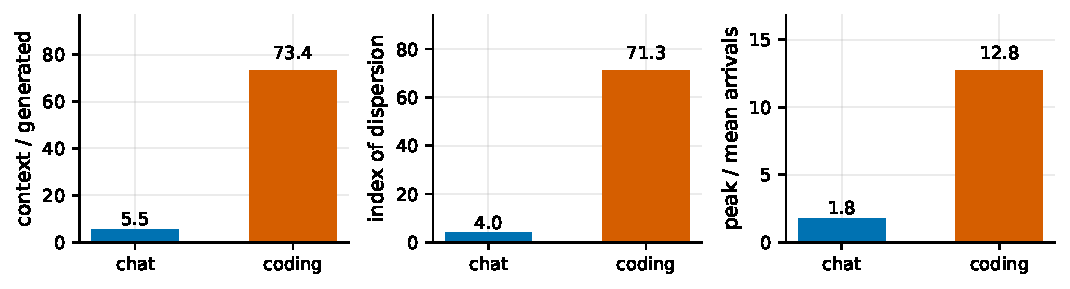
\includegraphics[width=\columnwidth]{figs/f1_trace_contrast.pdf}
\caption{Measured properties of the two Azure traces.}
\label{fig:traces}
\end{figure}

\subsection{Three zeroes, one latent value}

GPU utilisation, queue depth, and active-KV utilisation are sensible signals
for submitted requests. A parked program is outside that interface. Yet a
cache hit can make its next turn much cheaper. We denote a program's cached
prefix by $c_i$ and the fraction still present when it returns by $q_i\in[0,1]$.
Its latent recompute liability is
\begin{equation}
  L_i = \frac{(1-q_i)c_i}{R_{\mathrm{prefill}}}.
  \label{eq:liability}
\end{equation}
Neither $q_i$ nor the program's probability of returning is exported by the
three native autoscaling signals. Counting programs alone supplies neither.

\section{Hardware Validation}
\label{sec:validation}

\subsection{Setup}

We ran vLLM~0.25.1 with prefix caching enabled, using the Qwen2.5-14B
Instruct checkpoint on one device reported as RTX~4090 with 49,140~MiB.
The server reported capacity for 75,216 KV-cache tokens. Each point has three
repetitions unless noted. The repository contains the exact scripts, raw CSVs,
server logs, and a machine-readable summary.

\begin{figure*}[t]
\centering
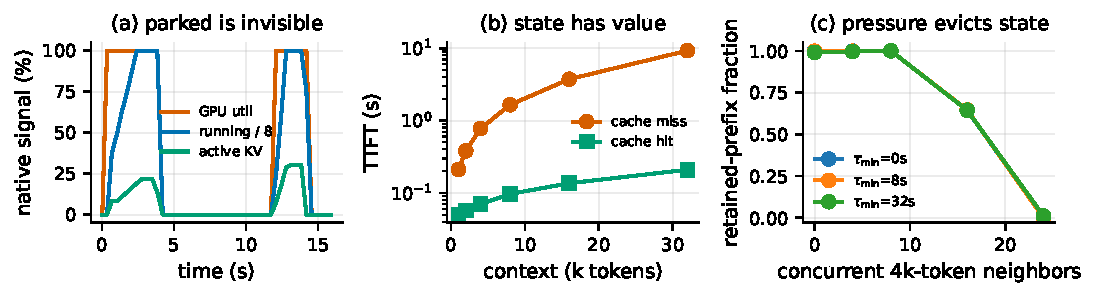
\includegraphics[width=\textwidth]{figs/f8_vllm_measured.pdf}
\caption{Hardware validation. (a) During tool-call intervals, all three native
signals drop to zero. (b) Cache loss has a context-proportional TTFT cost.
(c) A parked prefix survives elapsed time but not sufficient concurrent
pressure; the score estimates the retained fraction from hit/miss TTFT.}
\label{fig:measured}
\end{figure*}

\subsection{V1: price of a prefix}

We issue the same prefix twice for a hit and a distinct prefix for a miss.
At 1k tokens, the mean miss--hit penalty is 0.161~s; at 32k it is 9.028~s
and the hit is $44.2\times$ faster. A linear fit gives 0.286~s per 1k tokens
with $R^2=0.989$. The state is valuable even though it is not reserved.

\subsection{V2: the assumption that failed}

Eight sessions alternate model calls with 8~s tool sleeps while DCGM and the
vLLM Prometheus endpoint are sampled. Across 114 samples in which all sessions
are parked, mean GPU utilisation, running requests, waiting requests, and
active-KV utilisation are all exactly zero. When any session computes, the
corresponding means are 93.5\% GPU, 5.96 running, 0.62 waiting, and 29.5\%
active KV. Thus KV-util does not rescue observability of parked state.

\subsection{V3--V4: calibration}

At concurrency $k\in\{1,2,4,8,16,32\}$, per-sequence output rate fits
\begin{equation}
  r(k)=\frac{R}{k+k_{1/2}}
  \label{eq:batch}
\end{equation}
with $R=156.19$, $k_{1/2}=4.606$, and $R^2=0.99995$. The original assumed
$k_{1/2}=16$, so its batching model was materially too optimistic. Three clean
server process starts with a warm host page cache take 38.163, 38.141, and
38.161~s (mean 38.155~s). This is not a disk-cold or 70B cold start.

\subsection{P1: survival under delay and pressure}

We park a 16k-token target, immediately issue
$N\in\{0,4,8,16,24\}$ distinct 4k-token neighbors, and then wait if necessary
so the total park interval reaches the minimum target
$\tau_{\min}\in\{0,8,32\}$~s before probing. We normalize probe TTFT between
the same-trial hit and miss to estimate retained prefix fraction. All 45 trials
completed. At $N\le8$, retention is essentially one; at $N=16$, it is 0.645;
and at $N=24$, it is approximately zero. The pressure work itself takes about
12.2~s and 18.2~s at $N=16$ and $N=24$, respectively, so it overruns the
0/8-s minimum targets. Across the distinct elapsed times available at each
pressure level, allocation pressure rather than wall-clock age determines
survival in this range.

This result also exposes partial eviction. The measured capacity is 75,216
tokens; a 16k target plus sixteen 4k neighbors exceeds it by about 4.8k tokens,
consistent with a partial rather than all-or-nothing miss.

\section{Corrected Method}

\subsection{Real and constructed inputs}

Arrival time, context length, and generated length come directly from the Azure
traces. The traces contain neither program identifiers nor tool durations. We
construct programs of $T\in\{1,4,16,64\}$ turns and sweep mean tool delay
$\tau\in\{0,8,30\}$~s. $T=1,\tau=0$ is the unmodified request-level control.
Context accumulates across constructed turns. We use seed 20260720.

\subsection{State model and service calibration}

Each replica separately tracks active KV allocation and reclaimable cached
content. A completed turn releases its active allocation but leaves its prefix
as LRU content. New active blocks reclaim the oldest parked prefixes at token
granularity. Scale-in removes only idle replicas and discards any cached content
on them. On return, the program prefills only the missing part of its prefix.

Defaults use the measured 75,216-token capacity, $k_{1/2}=4.606$, and
38.155~s process cold start. Jointly fitting V1 and V3 gives a service rate of
19,607 token-equivalents/s and decode weight 94.28 relative to prefill. Maximum
batch is 32. E7 explicitly sweeps capacity, batch, and policy target.

We simulate 2,400~s of arrivals, exclude a 300~s warm-up from scoring, then
stop arrivals and drain for the larger of 600~s or a workload-derived bound.
This drain is essential: scoring only to the last arrival mechanically labels
late long programs as failures. Every admitted turn completes in the final
runs, so goodput is one and does not separate policies.

The SLO is per-turn slowdown at most three. For each workload we search for the
smallest static cluster achieving at least 95\% SLO attainment. Dynamic cost is
reported as GPU-seconds relative to that reference. Unfinished admitted work,
if any, is counted as an SLO failure.

\subsection{Policies}

We implement HPA on GPU utilisation (70\% target and 300~s scale-down
stabilisation), KEDA on waiting requests, KV-util on active KV (80\% target),
a Holt arrival forecaster, and tabular Q-learning with and without parked count
in its state~\cite{gari,barrett}. The candidate \sys policy uses
\begin{equation}
N=\max\!\left(
\left\lceil\frac{\mathrm{running}+\mathrm{queued}+\mathrm{parked}}
{B\theta}\right\rceil,
\left\lceil\frac{\mathrm{active\ KV}}{K\theta}\right\rceil\right).
\label{eq:parkaware}
\end{equation}
It is retained unchanged as the direct test of the original idea. Under the
corrected mechanism, its parked term is a conservative seat reservation, not a
measurement of pinned memory.

\section{Results}

\subsection{Parked work is common and natively invisible}

On a fixed eight-replica cluster, the simulated parked fraction is 60.2\% at
$(T,\tau)=(4,4)$, 89.5\% at $(8,8)$, and 93.1\% at $(16,8)$.
At those points, respectively 16.2\%, 27.6\%, and 24.3\% of post-warm-up
samples contain parked programs while running, GPU, and active-KV signals are
all zero. Figure~\ref{fig:parking} distinguishes how much work is parked from
how often its invisibility is complete.

\begin{figure}[t]
\centering
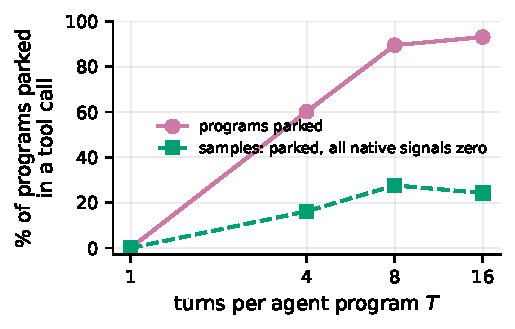
\includegraphics[width=.78\columnwidth]{figs/f2_parked_fraction.pdf}
\caption{Simulated parked fraction and completely invisible parked intervals
on a fixed cluster. Reclaimable cache is tracked internally but is not a native
autoscaling signal.}
\label{fig:parking}
\end{figure}

\subsection{Counting parked programs is not a robust policy}

\begin{figure*}[t]
\centering
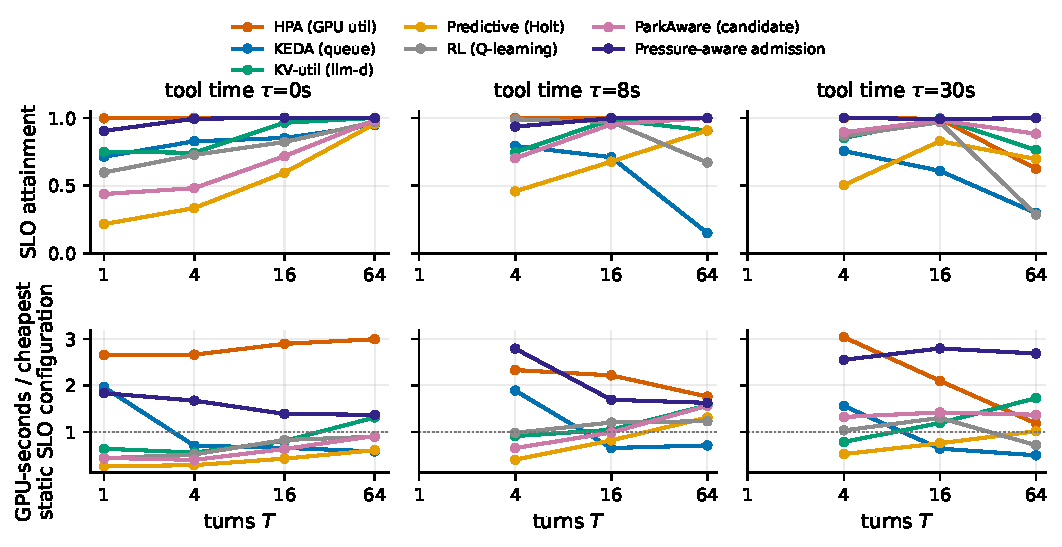
\includegraphics[width=\textwidth]{figs/f3_main_slo.pdf}
\caption{SLO attainment and GPU cost relative to the cheapest static
SLO-meeting cluster. The corrected model yields no universal dynamic-policy
winner; ParkAware is a candidate baseline, not ``ours'' with a claimed win.}
\label{fig:main}
\end{figure*}

\begin{table}[t]
\centering\small
\caption{Mean over the six coding-trace agentic points ($T>1,\tau>0$).}
\label{tab:main}
\begin{tabular}{lrr}
\toprule
Policy & SLO attainment & GPU / static \\
\midrule
HPA (GPU) & \textbf{0.935} & 1.914 \\
KEDA (queue) & 0.519 & 0.954 \\
KV-util & 0.931 & 1.339 \\
Predictive & 0.692 & 0.925 \\
RL (Q-learning) & 0.720 & 0.998 \\
RL + parked & 0.651 & 0.921 \\
\sys candidate & 0.909 & 1.430 \\
\bottomrule
\end{tabular}
\end{table}

Table~\ref{tab:main} reverses the uploaded paper's headline. \sys beats HPA
on three of six agentic points and KV-util on two, but loses in the mean. It
beats KEDA on five of six, yet usually spends more GPU time. No dynamic policy
simultaneously matches the cheapest static SLO configuration and costs less on
average. The appropriate conclusion is not that native metrics are sufficient:
rather, a parked count by itself is also insufficient.

The result varies by regime. At $(T,\tau)=(4,8)$, HPA attains 1.000 and
\sys 0.693. At $(16,30)$, \sys attains 1.000 and HPA 0.987. At $(64,8)$,
KV-util and \sys both attain approximately 1.000 while HPA is 0.764. Such crossovers are
exactly what a single occupancy proxy should produce when prefix value depends
on context size, return timing, cache pressure, and service batching.

\subsection{Pressure dominates scale-in damage}

\begin{figure}[t]
\centering
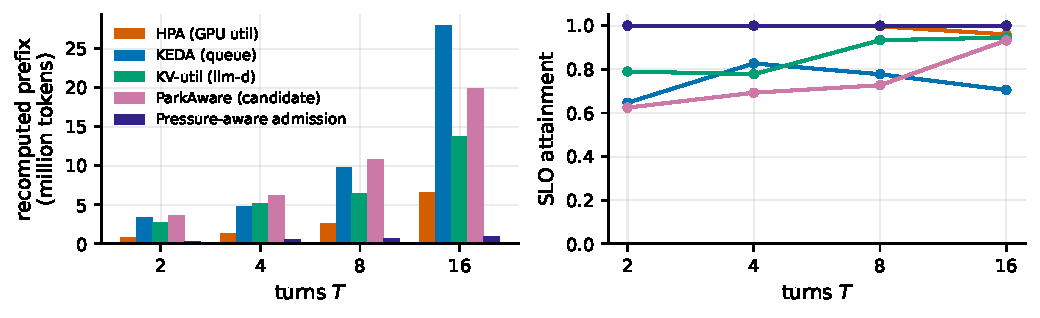
\includegraphics[width=\columnwidth]{figs/f4_scalein_damage.pdf}
\caption{Recomputed prefix tokens and SLO on the coding trace. Recompute
includes partial pressure eviction and cache loss on scale-in.}
\label{fig:damage}
\end{figure}

At $T=8,\tau=8$, HPA recomputes 2.56M tokens, of which only 0.218M are
attributed to scale-in. KEDA, KV-util, and \sys recompute 9.82M, 6.44M, and
10.76M tokens respectively; their scale-in components are only 0.532M,
0.163M, and 0.278M. Thus routine cache pressure is the dominant source of lost
prefix work in this model. The old equation that charged every parked context
only when a replica was removed described the wrong mechanism.

\subsection{Cold start and workload change the ordering}

At the measured 38.155~s process cold start, HPA, KEDA, Predictive, and
\sys attain 0.997, 0.777, 0.448, and 0.727 at $(T,\tau)=(8,8)$.
At 180~s they attain 0.650, 0.635, 0.303, and 0.537. The original monotone
ParkAware advantage does not survive correction: KEDA is best among these four
at 180~s, and HPA is best at the measured point.

On the conversation trace constructed as $T=8,\tau=8$, HPA attains 1.000,
KV-util 0.907, and \sys 0.972; KEDA falls to 0.241. On the coding trace at the
same point, the values are 0.997, 0.933, and 0.727 for the first, third, and
fourth policies. A program-level policy cannot be evaluated independently of
the token and arrival distribution beneath the constructed program structure.

\begin{figure}[t]
\centering
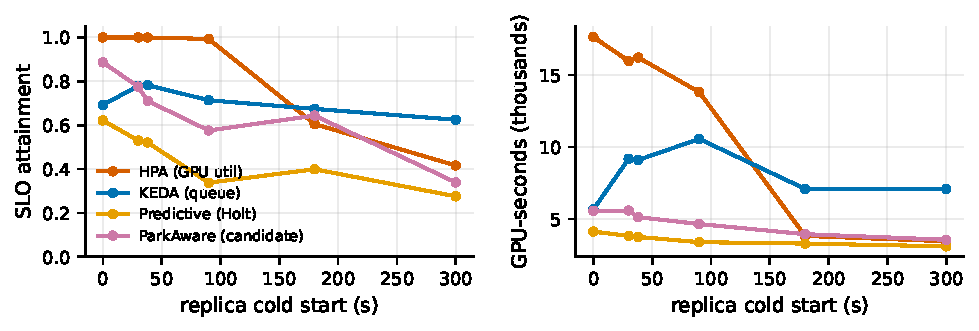
\includegraphics[width=\columnwidth]{figs/f5_coldstart.pdf}
\caption{Cold-start sensitivity at $T=8,\tau=8$. The measured 14B point is
38.155~s; larger values are sensitivity cases, not measurements.}
\label{fig:cold}
\end{figure}

\subsection{Sensitivity confirms that no scalar signal is enough}

At measured capacity and batch 32, HPA/KV-util/\sys attain
0.997/0.933/0.727. At batch 16 the same values are
1.000/0.932/0.940; at batch 64, 0.996/0.828/0.626. Sweeping capacity from
31k to 500k also changes the ordering, and changing \sys's target from 0.5 to
0.9 moves its attainment from 0.831 to 0.638. The candidate is sensitive to
the resource regime and control target, contrary to the original robustness
claim.

\section{Implications}

\paragraph{Expose cache state, not only allocation.}
Active-KV utilisation correctly reports allocated blocks, but an autoscaler
also needs the amount, age, ownership, and eviction priority of reclaimable
prefix content. Conflating the two would make admission control unsafe;
exporting both would preserve the distinction.

\paragraph{Value is probabilistic.}
A parked prefix is worth approximately its miss penalty times the probability
that the program returns before pressure evicts it. Tool type, transcript size,
recent reuse, and cache competition may predict that value. A raw parked count
assigns the same value to a 1k prefix and a 32k prefix despite a measured
56-fold difference in recompute penalty.

\paragraph{Scale-in should be cache-aware, not cache-fearing.}
Scale-in is destructive when it targets a replica with valuable surviving
prefixes, but keeping a replica for already-evicted or unlikely-to-return state
wastes capacity. A practical controller should coordinate replica draining
with prefix placement and eviction metadata rather than prohibit scale-in
based on program count.

\section{Threats to Validity}
\label{sec:threats}

\textbf{Single hardware configuration.} Four modelling assumptions are
measured on a single vLLM instance. One assumption was falsified by that
measurement and the model corrected accordingly. Results may differ across
engines, versions, models, cache managers, and hardware. V4 measures a process
restart with warm host page cache, not a machine reboot or disk-cold start.

\textbf{Constructed program structure.} Azure supplies request records, not
agent identities or tool intervals. Our $T$ and $\tau$ are constructed. Sweeps
and a $T=1$ control expose, but do not eliminate, this limitation.

\textbf{Simulator rather than cluster replay.} Hardware measurements calibrate
the mechanism and service curve; E2--E7 are still simulations. The model uses
LRU pressure, one model per replica, and simplified placement. Production
schedulers may migrate, preempt, offload, or explicitly pin cache state.

\textbf{Policy implementations.} The policies follow their documented signal
and standard control forms, but deployment-specific tuning can change results.
The tabular RL baseline is deliberately conventional, not a claim about all
learning-based controllers. We present \sys as a falsified candidate rather
than a production recommendation.

\section{Related Work}

PagedAttention and vLLM make KV management efficient within a serving
instance~\cite{vllm}. Agent-serving systems increasingly schedule whole
programs rather than isolated requests; Autellix, for example, uses cumulative
program service time~\cite{autellix}. This work addresses the interface between
that program state and cluster-level elasticity.

LLM autoscaling work optimizes token-aware or disaggregated serving.
TokenScale scales on token velocity, while ServerlessLLM attacks model-loading
cold start directly~\cite{tokenscale,serverlessllm}. DistServe and DynamoLLM
optimize cluster organization and goodput~\cite{distserve,dynamollm}. Our
measurement shows that active request metrics omit a distinct object:
reclaimable, application-owned prefix value between requests.

Classical elasticity separates reactive, proactive, and learning-based
controllers~\cite{herbst,gari}. RL resource allocation has a long history
\cite{barrett}. Our corrected result is compatible with that literature's main
lesson: policy quality depends on the state representation. Here, neither
native active-resource signals nor a parked-program count represents prefix
survival and value.

\section{Conclusion}

A parked agent does not hard-hold KV in native vLLM, but it may retain a cheap
path back into execution. That path has measurable value, is invisible to
native autoscaling metrics, and disappears under cache pressure. Correcting
this distinction invalidates both our original mechanism and its claimed
ParkAware advantage. The robust conclusion is narrower and more useful:
agentic autoscaling needs an explicit signal for reclaimable prefix state and
its reuse probability. We release the failed assumption and corrected negative
result so subsequent designs can start from the measured system rather than a
convenient fiction.

\appendix
\section{Sensitivity Figure}

\begin{figure}[h]
\centering
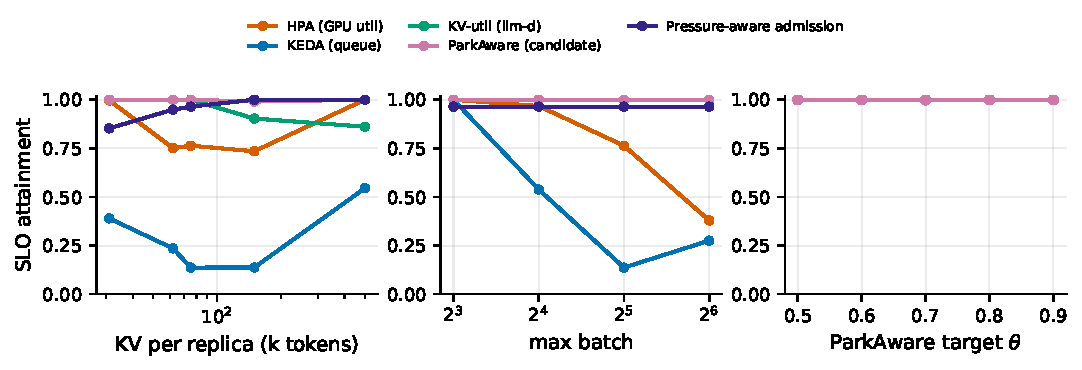
\includegraphics[width=\columnwidth]{figs/f7_sensitivity.pdf}
\caption{Sensitivity at $T=8,\tau=8$: KV capacity, maximum batch, and the
candidate ParkAware target.}
\label{fig:sensitivity}
\end{figure}

\bibliographystyle{ACM-Reference-Format}
\begin{thebibliography}{99}
\small
\bibitem{splitwise} P.~Patel et al. Splitwise: Efficient generative LLM
inference using phase splitting. In \emph{ISCA}, 2024. Traces:
\url{https://github.com/Azure/AzurePublicDataset}.
\bibitem{react} S.~Yao et al. ReAct: Synergizing reasoning and acting in
language models. In \emph{ICLR}, 2023.
\bibitem{vllm} W.~Kwon et al. Efficient memory management for large
language model serving with PagedAttention. In \emph{SOSP}, 2023.
\bibitem{autellix} M.~Luo et al. Autellix: An efficient serving engine for
LLM agents as general programs. arXiv:2502.13965, 2025.
\bibitem{tokenscale} R.~Lai et al. TokenScale: Timely and accurate
autoscaling for disaggregated LLM serving with token velocity.
arXiv:2512.03416, 2025.
\bibitem{serverlessllm} Y.~Fu et al. ServerlessLLM: Low-latency serverless
inference for large language models. In \emph{OSDI}, 2024.
\bibitem{herbst} N.~Herbst, S.~Kounev, R.~Reussner. Elasticity in cloud
computing: What it is, and what it is not. In \emph{ICAC}, 2013.
\bibitem{barrett} E.~Barrett, E.~Howley, J.~Duggan. Applying reinforcement
learning towards automating resource allocation and application scalability
in the cloud. \emph{Concurrency and Computation}, 25(12), 2013.
\bibitem{gari} Y.~Gar\'i et al. Reinforcement learning-based application
autoscaling in the cloud: A survey. \emph{Engineering Applications of
Artificial Intelligence}, 2021.
\bibitem{polar} Polar: Agentic RL on any harness at scale.
arXiv:2605.24220, 2026.
\bibitem{dynamollm} J.~Stojkovic et al. DynamoLLM: Designing LLM inference
clusters for performance and energy efficiency. In \emph{HPCA}, 2025.
\bibitem{distserve} Y.~Zhong et al. DistServe: Disaggregating prefill and
decoding for goodput-optimized LLM serving. In \emph{OSDI}, 2024.
\end{thebibliography}

\end{document}
